\subsection{Source Control Management}
% Auto-generate the TOC slide(s)
\begin{frame}
  \tableofcontents[currentsection, currentsubsection]
  %\tableofcontents
\end{frame}


\setbeamercolor{normal text}{fg=gray,bg=}
\setbeamercolor{alerted text}{fg=black,bg=}

\begin{frame}
Why use source control managment?
\usebeamercolor{normal text}
  \begin{itemize}
    \item \alert<+>{Traceability, know when things were added.}
    \item \alert<+>{Reproducibility, know what code was run when.}
    \item \alert<+>{Collaboration, allow contributions without risking code breakage.}
  \end{itemize}
\end{frame}

\subsubsection{Local Source Control Management}
\begin{frame}
\begin{columns}[c]
\column{2in}
\framebox{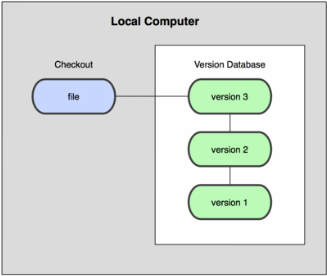
\includegraphics[scale=.5]{../figures/git/local_scm.png}}
\column{2in}
\only<1-3>{
\usebeamercolor{normal text}
\begin{itemize}
\item \alert<+>{Edit and revise local files.}
\item \alert<+>{Keep versions of the file that can be ``checked out''.}
\item \alert<+>{Use smart tools to see differences in the files.}
\end{itemize}
}
\only<4>{
Examples:
\begin{itemize}
\item{SCCS (1972)}
\item{RCS (1982)}
\end{itemize}
}
\end{columns}
\end{frame}

\subsubsection{Centralized Source Control Management}
\begin{frame}
\begin{columns}[c]
\column{2in}
\only<1-3>{
\usebeamercolor{normal text}
\begin{itemize}
\item \alert<+>{Same interactions as local SCM.}
\item \alert<+>{Diffs stored on central resource for access management.}
\item \alert<+>{Easy to work on same code at the same time.}
\end{itemize}
}
\only<4>{
Examples:
\begin{itemize}
\item{CVS (1989)}
\item{SVN (2000)}
\item{ClearCase}
\item{Perforce}
\end{itemize}
}
\column{2.5in}
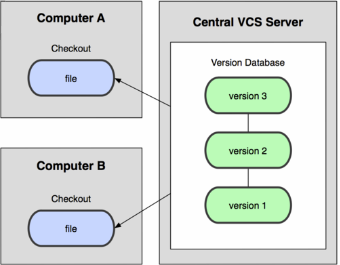
\includegraphics[scale=.5]{../figures/git/centralized_scm.png}
\end{columns}
\end{frame}

\subsubsection{Distributed Source Control Management}
\begin{frame}
\begin{columns}
\column{2in}
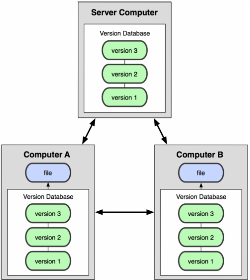
\includegraphics[scale=.5]{../figures/git/distributed_scm.png}
\column{2in}
\only<1-3>{
\usebeamercolor{normal text}
\begin{itemize}
\item \alert<+>{Edit and revise local files, but also keep version database local}
\item \alert<+>{Easy to give full repository to collaborators.}
\item \alert<+>{Completely distributed allowing for a several workflow styles.}
\end{itemize}
}
\only<4>{
Examples:
\begin{itemize}
\item{Bitkeeper (2000)}
\item{Darcs (2003)}
\item{Git (2005)}
\item{Bazaar (2005)}
\item{Mercurial (2005)}
\end{itemize}
}
\end{columns}
\end{frame}

\begin{frame}
\begin{center}
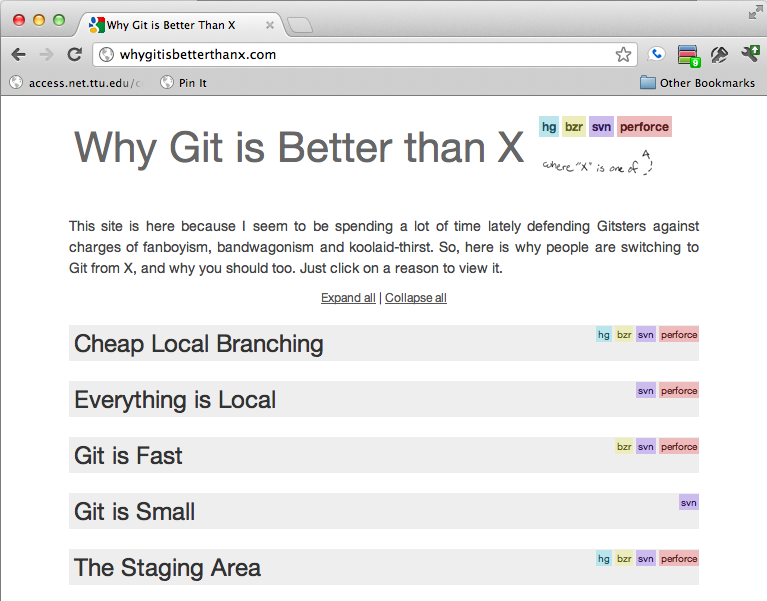
\includegraphics[scale=.4]{../figures/git/whygitisbetter.png}
\end{center}
\end{frame}
